% Provenance (never printed): old seconde/premiere S material on the
% atmosphere (storms, cyclones, the energy of the water cycle) and the
% natural-hazard themes of SVT; see sources/book2/PROVENANCE.md. Tracks,
% genesis statistics and the pressure--wind relation are computed in
% figdata/grade-10/cyclones.py from IBTrACS v04r01; the surge, thunder and
% energy numbers in the same script.
\chapter{तूफ़ान और उष्णकटिबंधीय चक्रवात}\label{ch:g10:storms-and-cyclones}

गर्मियों की एक तपती दोपहर तूफ़ान में बदल जाती है। आकाश काला पड़ जाता है, ठंडी हवा का एक
झोंका गली को बुहार देता है, एक चमक बादलों को रोशन कर देती है --- और आप गिनने लगते हैं:
एक, दो, तीन, \ldots{} नौ सेकंड बाद गरज लुढ़कती है। तूफ़ान लगभग तीन किलोमीटर दूर
है। एक घंटे में वह गुज़र चुका होगा, और हवा ठंडी और स्वच्छ होगी। गरम उष्णकटिबंधीय
महासागरों के ऊपर यही सामग्री --- गरम, नम हवा जो ऊपर उठती है और संघनित होती है ---
बिल्कुल दूसरे आकार के तूफ़ानों में संगठित हो सकती है: \omterm{def:g10:storms-and-cyclones:tropical-cyclone}{उष्णकटिबंधीय चक्रवात}, सैकड़ों
किलोमीटर चौड़े, जो कई दिन चलते हैं और इतनी तेज़ पवनें लाते हैं कि जंगल धराशायी हो जाएँ, और
समुद्र का ऐसा उभार कि पूरे के पूरे तट डूब जाएँ। यह अध्याय \omterm{def:g10:storms-and-cyclones:thunderstorm}{तड़ित-झंझाओं}, \omterm{def:g10:storms-and-cyclones:tornado}{टॉरनेडो} और
\omterm{def:g10:storms-and-cyclones:tropical-cyclone}{उष्णकटिबंधीय चक्रवातों} को देखता है, और यह भी कि उनकी ऊर्जा कहाँ से आती
है।

\begin{safety}
यदि आपको गरज सुनाई देती है, तो \omterm{def:g10:storms-and-cyclones:lightning}{तड़ित} आप तक पहुँच सकती है। किसी इमारत में या किसी
बंद कार में जाइए और अंतिम गरज के काफ़ी देर बाद तक वहीं रहिए। किसी अकेले पेड़ के नीचे
कभी शरण न लीजिए, और पहाड़ियों की चोटियों, खुले मैदानों और पानी से दूर रहिए।
\end{safety}

\begin{recall}
वायु राशियाँ, वाताग्र, अवदाब (निम्न दाब के क्षेत्र) और प्रतिचक्रवात
मौसम मानचित्रों पर समदाब रेखाओं से, यानी समान दाब की रेखाओं से, बनाए जाते हैं (पुस्तक 1,
कक्षा 8)। प्राकृतिक संकट ऐसी प्राकृतिक घटना है जो लोगों को और उनके बनाए
को हानि पहुँचा सकती है (पुस्तक 1, कक्षा 5)। ध्वनि हवा में लगभग
\qty{340}{m/s} से चलती है, प्रकाश लगभग तुरंत (भौतिकी की पुस्तकें)। ऊपर उठती गरम, नम
हवा ठंडी होती है, अपने \omterm{def:g10:why-clouds-form:condensation-level}{संघनन तल} पर संघनित होकर बादल बनती है और
\omterm{def:g10:earth-energy-budget:latent-heat}{गुप्त ऊष्मा} छोड़ती है; संतृप्त हवा अक्सर अस्थिर होती है
(\cref{ch:g10:why-clouds-form})।
\end{recall}

\section{तड़ित-झंझा}

\begin{definition}[तड़ित-झंझा]\label{def:g10:storms-and-cyclones:thunderstorm}
\emph{तड़ित-झंझा}\index{तड़ित-झंझा} किसी कपासी वर्षी मेघ से उत्पन्न ऐसा तूफ़ान है
जिसमें \omterm{def:g10:storms-and-cyclones:lightning}{तड़ित} और गरज होती है, सामान्यतः तेज़ बौछारें
और पवन के झोंके होते हैं, कभी-कभी ओले भी।
\end{definition}

\omterm{def:g10:storms-and-cyclones:thunderstorm}{तड़ित-झंझा} अस्थिर, नम हवा से पनपती है। अपनी पहली अवस्था में एक कपासी मेघ
तेज़ ऊर्ध्व धारा से पोषित होकर ऊपर की ओर बढ़ता है; संघनन \omterm{def:g10:earth-energy-budget:latent-heat}{गुप्त ऊष्मा} छोड़ता है
और ऊपर उठती हवा को उसके परिवेश से अधिक गरम रखता है। अपनी परिपक्व अवस्था में
बादल बहुत ऊपर की \omterm{def:g10:why-clouds-form:stability}{स्थिर वायु} तक पहुँचता है और एक निहाई के रूप में फैल जाता है;
बूँदें और ओले इतने बड़े हो जाते हैं कि गिर सकें, और गिरती वर्षा अपने साथ
ठंडी हवा नीचे खींच लाती है: एक अधो धारा, जो ज़मीन पर एक ठंडे झोंका-वाताग्र के रूप में
फैल जाती है। अपनी अंतिम अवस्था में अधो धारा पूरे बादल पर हावी हो जाती है,
गरम नम हवा की आपूर्ति काट देती है, और तूफ़ान बरसकर स्वयं को
समाप्त कर लेता है।

\begin{omfigure}
\begin{tikzpicture}[font=\footnotesize, >={Stealth[length=2mm]}]
  \foreach \dx/\title in {0/{1. बढ़ता हुआ}, 4.6/{2. परिपक्व}, 9.2/{3. बिखरता हुआ}}
    \node[anchor=north] at (\dx+1.6,-0.15) {\title};
  \draw[thick, black!60] (-0.3,0) -- (12.9,0);
  % stage 1: a tall cumulus
  \pic[scale=1.4, transform shape] at (1.6,1.2) {puffycloud};
  \pic[scale=1.1, transform shape] at (1.6,2.0) {puffycloud};
  \foreach \x in {1.2,1.6,2.0} \draw[->, thick, omThm!80!black] (\x,0.2) -- (\x,2.6);
  % stage 2: cumulonimbus with anvil
  \fill[black!8, draw=black!50] (5.0,1.0) -- (4.9,4.0) -- (4.2,4.4) -- (8.0,4.6) -- (7.4,4.0) -- (7.2,1.0) -- cycle;
  \draw[->, thick, omThm!80!black] (5.5,0.2) -- (5.5,4.2);
  \draw[->, thick, omThm!80!black] (5.9,0.2) -- (5.9,4.2);
  \draw[->, thick, omDef!80!black] (6.7,3.4) -- (6.7,0.3) -- (7.6,0.3);
  \foreach \x in {6.4,6.85,7.05} \draw[omDef!50] (\x,0.95) -- (\x-0.1,0.1);
  \node[anchor=west, align=left] at (8.0,4.6) {निहाई};
  \node[anchor=west, align=left, omDef!80!black] at (7.65,0.45) {झोंका-वाताग्र};
  % stage 3: dissipating
  \fill[black!8, draw=black!50] (9.7,1.2) -- (9.6,3.6) -- (9.0,4.0) -- (12.6,4.1) -- (12.0,3.6) -- (11.8,1.2) -- cycle;
  \foreach \x in {10.3,10.9,11.5} \draw[->, thick, omDef!80!black] (\x,3.2) -- (\x,0.3);
  \foreach \x in {10.6,11.2} \draw[omDef!50] (\x,1.15) -- (\x-0.1,0.1);
  % legend
  \draw[->, thick, omThm!80!black] (0,5.0) -- (0,5.5); \node[anchor=west] at (0.1,5.25) {गरम ऊर्ध्व धारा};
  \draw[->, thick, omDef!80!black] (3.2,5.5) -- (3.2,5.0); \node[anchor=west] at (3.3,5.25) {ठंडी अधो धारा};
\end{tikzpicture}

{\small \omterm{def:g10:storms-and-cyclones:thunderstorm}{तड़ित-झंझा} की तीन अवस्थाएँ (व्यवस्था-चित्र, पैमाने पर नहीं): ऊर्ध्व
धाराओं से पोषित बढ़ता कपासी मेघ; परिपक्व कपासी वर्षी मेघ, अपनी निहाई, अपनी
ऊर्ध्व धारा और वर्षा द्वारा नीचे खींची गई अधो धारा के साथ; बिखरता
तूफ़ान, केवल अधो धारा।}
\end{omfigure}

बादल के भीतर, हवा द्वारा ऊपर-नीचे ले जाए जाते बर्फ़ के कणों की टक्करें
विद्युत आवेशों को अलग करती हैं: बादल आवेशित हो जाता है, सामान्यतः
तले पर ऋणात्मक और शीर्ष पर धनात्मक, और उसके नीचे की ज़मीन
भी अपना एक आवेश ग्रहण कर लेती है।

\begin{definition}[तड़ित]\label{def:g10:storms-and-cyclones:lightning}
\emph{तड़ित}\index{तड़ित} एक विशाल विद्युत चिंगारी है जो किसी तूफ़ान के
आवेशित क्षेत्रों को अनावेशित करती है, बादल के भीतर, बादलों के बीच, या
बादल और ज़मीन के बीच। वह हवा की एक सँकरी नली को इतनी अचानक गरम करती है कि
हवा एक आघात के साथ फैलती है: इस प्रसार की ध्वनि \emph{मेघगर्जन} (गरज) है।
\end{definition}

\begin{omfigure}
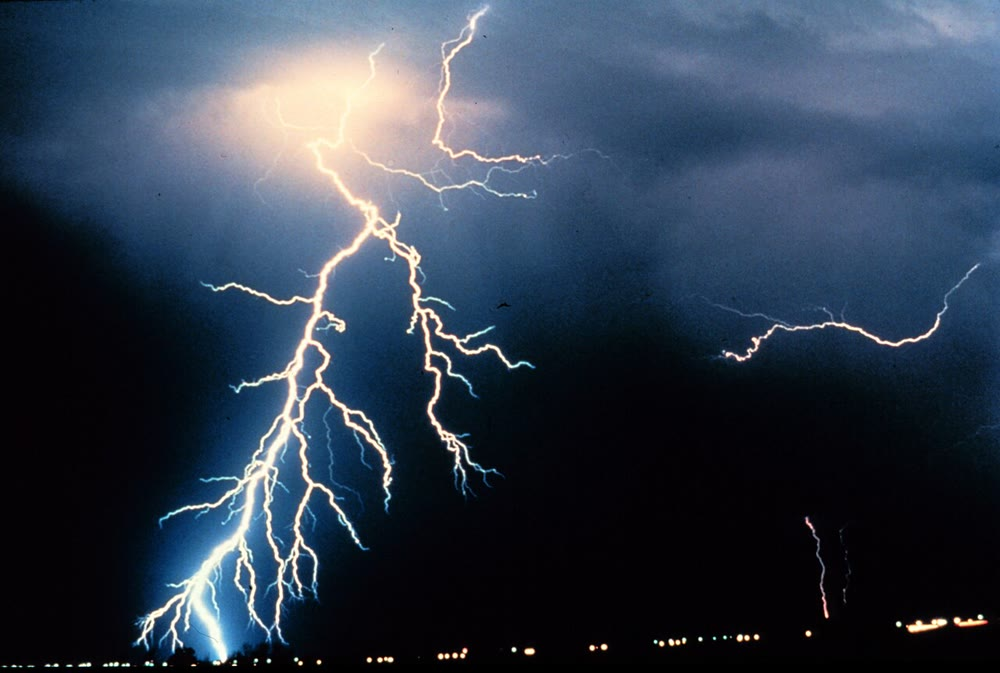
\includegraphics[width=0.62\linewidth]{images/book2/g10-noaa-lightning.jpg}

{\small रात की एक \omterm{def:g10:storms-and-cyclones:thunderstorm}{तड़ित-झंझा} के दौरान बादलों के बीच और बादल से ज़मीन तक
\omterm{def:g10:storms-and-cyclones:lightning}{तड़ित} के प्रहार। फ़ोटो: सी॰~क्लार्क, NOAA की राष्ट्रीय
प्रचंड तूफ़ान प्रयोगशाला (सार्वजनिक डोमेन)।}
\end{omfigure}

पूरे ग्रह पर प्रकाश की चमकें गिनने वाले उपग्रह प्रति वर्ष लगभग
1.4 अरब \omterm{def:g10:storms-and-cyclones:lightning}{तड़ित-चमकें} पाते हैं, यानी हर सेकंड 44।
% ledger: christian:flash-rate

\begin{method}[चमक से गरज तक: तूफ़ान की दूरी]\label{met:g10:storms-and-cyclones:distance}
\begin{enumerate}
  \item चमक का प्रकाश व्यवहार में तुरंत पहुँचता है; गरज
        ध्वनि की चाल से चलती है, \qty{20}{\degreeCelsius} पर लगभग
        \qty{343}{m/s}।
  \item चमक और गरज के बीच के सेकंड $t$ गिनिए।
  \item दूरी $343\,t$ मीटर है: हर तीन सेकंड के लिए लगभग
        \qty{1}{km}।
\end{enumerate}
\end{method}
% ledger: const:R, earth:Mmol (speed of sound computed in figdata/grade-10/cyclones.py)

\section{टॉरनेडो}

\begin{definition}[टॉरनेडो]\label{def:g10:storms-and-cyclones:tornado}
\emph{टॉरनेडो}\index{टॉरनेडो} ज़मीन को छूता हुआ, प्रचंड वेग से घूमता हवा का एक स्तंभ है,
जो किसी कपासी वर्षी मेघ के आधार से लटकता है।
\end{definition}

सबसे शक्तिशाली \omterm{def:g10:storms-and-cyclones:tornado}{टॉरनेडो} \emph{सुपरसेल} से आते हैं, यानी ऐसी \omterm{def:g10:storms-and-cyclones:thunderstorm}{तड़ित-झंझाओं} से जिनकी
ऊर्ध्व धारा समग्र रूप से घूमती है। \omterm{def:g10:storms-and-cyclones:tornado}{टॉरनेडो} छोटा और अल्पकालिक होता है: प्रायः कुछ
सौ मीटर चौड़ा, कुछ मिनट टिकने वाला, और लगभग \qty{5.6}{km} के औसत मार्ग वाला।
पर उसकी पवनें पृथ्वी की सतह पर सबसे तेज़ होती हैं: मई 1999 में ओक्लाहोमा के एक
\omterm{def:g10:storms-and-cyclones:tornado}{टॉरनेडो} में एक चलित रडार ने ज़मीन से ऊपर लगभग \qty{135}{m/s} (लगभग \qty{480}{km/h})
मापी। संयुक्त राज्य अमेरिका में किसी भी अन्य देश से अधिक \omterm{def:g10:storms-and-cyclones:tornado}{टॉरनेडो} आते हैं, लगभग 1200
प्रति वर्ष; जिन अन्य क्षेत्रों में वे बार-बार आते हैं उनमें कनाडा के प्रेयरी मैदान,
बांग्लादेश, उत्तरी अर्जेंटीना और दक्षिणी ब्राज़ील, और
ब्रिटेन शामिल हैं।
% ledger: spc:tornado

\begin{omfigure}
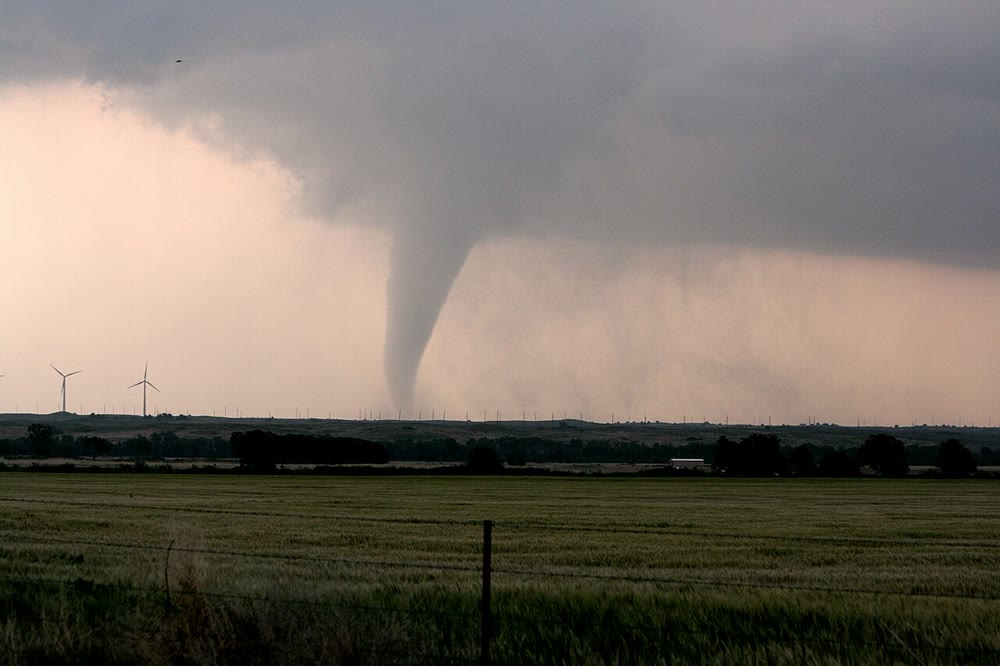
\includegraphics[width=0.62\linewidth]{images/book2/g10-noaa-tornado-kansas.jpg}

{\small मई 2008 में कैनसस के मैदानों के ऊपर एक \omterm{def:g10:storms-and-cyclones:tornado}{टॉरनेडो}: कीप तूफ़ानी बादल के आधार से
लटकी है। फ़ोटो: शॉन वॉ, NOAA की राष्ट्रीय
प्रचंड तूफ़ान प्रयोगशाला (सार्वजनिक डोमेन)।}
\end{omfigure}

\section{उष्णकटिबंधीय चक्रवात}

\begin{definition}[उष्णकटिबंधीय चक्रवात; आँख; आँख की दीवार]\label{def:g10:storms-and-cyclones:tropical-cyclone}
\emph{उष्णकटिबंधीय चक्रवात}\index{उष्णकटिबंधीय चक्रवात} सैकड़ों
किलोमीटर चौड़ा ऐसा तूफ़ान है जो गरम उष्णकटिबंधीय समुद्र के ऊपर निम्न दाब के एक
केंद्र के चारों ओर बनता है, जिसमें पवनें केंद्र की ओर सर्पिल रूप में भीतर घूमती हैं और
\omterm{def:g10:storms-and-cyclones:thunderstorm}{तड़ित-झंझाओं} की पट्टियाँ होती हैं। जब उसकी सतत पवनें \num{64}~नॉट, लगभग
\qty{119}{km/h}, तक पहुँचती हैं, तो उसे अटलांटिक और पूर्वी प्रशांत में हरिकेन कहते हैं,
पश्चिमी प्रशांत में टाइफ़ून, और हिंद महासागर तथा दक्षिणी प्रशांत में केवल
चक्रवात। उसका शांत, लगभग मेघरहित केंद्र
\emph{आँख}\index{आँख (चक्रवात)} है; उसके चारों ओर ऊँची \omterm{def:g10:storms-and-cyclones:thunderstorm}{तड़ित-झंझाओं} का वलय, जहाँ
पवनें सबसे तेज़ होती हैं, \emph{आँख की दीवार}\index{आँख की दीवार} है।
\end{definition}
% ledger: nhc:sshws

\begin{omfigure}
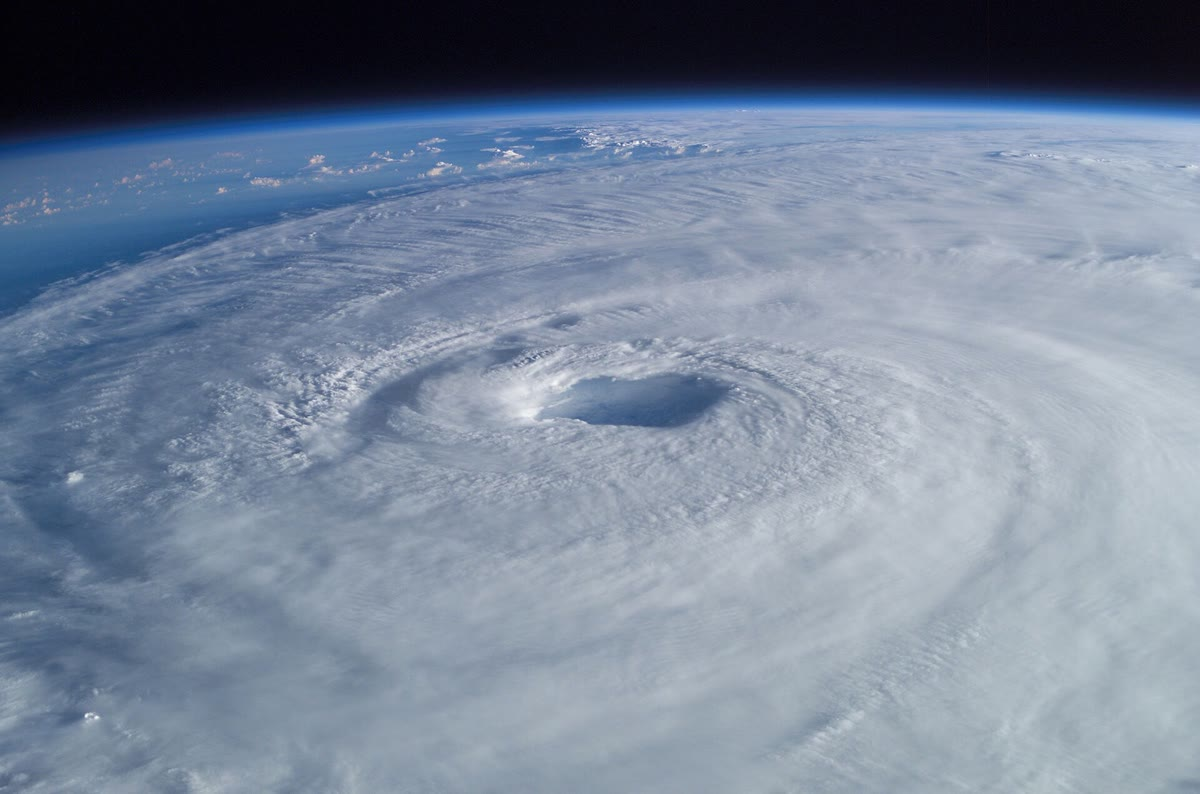
\includegraphics[width=0.78\linewidth]{images/book2/g10-nasa-hurricane-isabel.jpg}

{\small 15 सितंबर 2003 को हरिकेन इसाबेल, अंतरराष्ट्रीय अंतरिक्ष स्टेशन से एक
अंतरिक्ष यात्री द्वारा खींची गई फ़ोटो: \omterm{def:g10:storms-and-cyclones:tropical-cyclone}{आँख}, \omterm{def:g10:storms-and-cyclones:tropical-cyclone}{आँख की दीवार} और उनके चारों ओर बादलों
का सर्पिल। चित्र: माइक ट्रेंचर्ड, पृथ्वी विज्ञान एवं प्रतिबिंब विश्लेषण
प्रयोगशाला, NASA जॉनसन अंतरिक्ष केंद्र (सार्वजनिक डोमेन)।}
\end{omfigure}

समुद्र की सतह के पास नम हवा केंद्र के निम्न दाब की ओर भीतर बहती है।
पृथ्वी का घूर्णन चलती हवा को उत्तरी गोलार्ध में दाईं ओर मोड़ देता है:
सीधे केंद्र तक जाने के बजाय हवा उसके चारों ओर घूमती है, ऊपर से देखने पर
वामावर्त (दक्षिणी गोलार्ध में दक्षिणावर्त)। केंद्र के पास वह \omterm{def:g10:storms-and-cyclones:tropical-cyclone}{आँख की
दीवार} में ऊपर उठती है, संघनित होती है, और तूफ़ान के शीर्ष पर बाहर बह जाती है। \omterm{def:g10:storms-and-cyclones:tropical-cyclone}{आँख} में
थोड़ी हवा नीचे बैठती है, गरम होती है और सूख जाती है: आकाश साफ़ हो जाता है।

\begin{omfigure}
\begin{tikzpicture}[font=\footnotesize, >={Stealth[length=2mm]}]
  \fill[omDef!25] (-6,-0.4) rectangle (6,0);
  \node[anchor=north, omDef!80!black] at (0,-0.05) {गरम समुद्र};
  % rain bands
  \foreach \x/\h in {-5.0/1.6, -3.9/2.2, 3.9/2.2, 5.0/1.6}
    \fill[black!10, draw=black!45] (\x-0.35,0.4) -- (\x-0.3,\h) .. controls (\x-0.15,\h+0.35) and (\x+0.15,\h+0.35) .. (\x+0.3,\h) -- (\x+0.35,0.4) -- cycle;
  % eyewall towers and outflow canopy
  \fill[black!14, draw=black!50] (-2.4,0.4) -- (-2.5,4.0) -- (-5.8,4.3) -- (-5.6,4.7) -- (-1.0,4.9) -- (-0.75,4.0) -- (-0.8,0.4) -- cycle;
  \fill[black!14, draw=black!50] (2.4,0.4) -- (2.5,4.0) -- (5.8,4.3) -- (5.6,4.7) -- (1.0,4.9) -- (0.75,4.0) -- (0.8,0.4) -- cycle;
  % inflow, rise, outflow, eye subsidence
  \draw[->, thick, omThm!80!black] (-5.8,0.2) -- (-1.3,0.2) -- (-1.3,4.3) -- (-4.2,4.45);
  \draw[->, thick, omThm!80!black] (5.8,0.2) -- (1.3,0.2) -- (1.3,4.3) -- (4.2,4.45);
  \draw[->, thick, omDef!80!black] (0,4.3) -- (0,1.0);
  \node[anchor=south, align=center] at (0,5.0) {आँख: नीचे बैठती\\शुष्क हवा};
  \node[anchor=south east, align=right] at (-2.6,4.95) {आँख की दीवार};
  \node[anchor=west, align=left] at (-5.95,2.9) {वर्षा\\पट्टियाँ};
  \node[anchor=north, align=center] at (-3.6,0.15) {नम अंतर्वाह};
  \node[anchor=south east, align=right] at (5.8,4.95) {ऊपर बहिर्वाह};
  % plan view
  \begin{scope}[shift={(8.4,2.3)}]
    \draw[black!40] (0,0) circle (1.7);
    \foreach \a in {0,90,180,270}
      \draw[->, thick, omThm!80!black, domain=0:200, samples=30, variable=\t]
        plot ({(1.6-0.0045*\t)*cos(\a+\t)}, {(1.6-0.0045*\t)*sin(\a+\t)});
    \fill[white, draw=black!50] (0,0) circle (0.22);
    \node[anchor=north, align=center] at (0,-1.8) {ऊपर से देखने पर\\(उत्तरी गोलार्ध)};
  \end{scope}
\end{tikzpicture}

{\small अनुप्रस्थ काट में एक \omterm{def:g10:storms-and-cyclones:tropical-cyclone}{उष्णकटिबंधीय चक्रवात} (व्यवस्था-चित्र, ऊँचाई बहुत
बढ़ाकर दिखाई गई): नम हवा गरम समुद्र के ऊपर भीतर बहती है, \omterm{def:g10:storms-and-cyclones:tropical-cyclone}{आँख की दीवार} और
वर्षा पट्टियों में ऊपर उठती है, और शीर्ष पर बाहर बह जाती है; \omterm{def:g10:storms-and-cyclones:tropical-cyclone}{आँख} में थोड़ी हवा नीचे बैठती है।
दाएँ: उत्तरी गोलार्ध में ऊपर से देखने पर अंतर्वाह केंद्र के चारों ओर
वामावर्त घूमता है।}
\end{omfigure}

\omterm{def:g10:storms-and-cyclones:tropical-cyclone}{उष्णकटिबंधीय चक्रवातों} को गरम महासागर चाहिए: सतह पर कम से कम लगभग
\qty{27}{\degreeCelsius} का जल, जो लगभग \qty{46}{m} की गहराई तक
गरम हो। वे ठीक भूमध्य रेखा पर नहीं बनते, जहाँ पृथ्वी का
घूर्णन भीतर बहती हवा को कोई मोड़ नहीं देता: घूर्णन शुरू होने के लिए तूफ़ान को भूमध्य रेखा से
कम से कम लगभग \qty{480}{km} दूर होना चाहिए।
% ledger: aoml:formation

\begin{omfigure}
\begin{tikzpicture}
\begin{axis}[ommap, width=\linewidth, xtick={-180,-120,...,180}, ytick={-60,-30,0,30,60},
  ymin=-70, ymax=70, unbounded coords=jump]
\addplot[fill=omLithAlluv, draw=black!45, line width=0.2pt] table {figdata/out/shared-geo-land.dat};
\addplot[omThm!70, line width=0.25pt] table {figdata/out/grade-10-cyclones-tracks.dat};
\addplot[only marks, mark=*, mark size=0.45pt, omDef!90!black] table {figdata/out/grade-10-cyclones-genesis.dat};
\addplot[black!45, dashed, domain=-180:180] {0};
\end{axis}
\end{tikzpicture}

{\small \omterm{def:g10:storms-and-cyclones:tropical-cyclone}{उष्णकटिबंधीय चक्रवात}: 2015--2024 के मौसमों के सभी तूफ़ानों के मार्ग
(लाल), और वह स्थान जहाँ 1980--2024 के मौसमों के हर तूफ़ान ने
पहली बार उष्णकटिबंधीय तूफ़ान की तीव्रता प्राप्त की (नीले बिंदु)। आँकड़े: IBTrACS v04r01,
NOAA राष्ट्रीय पर्यावरण सूचना केंद्र।}
\end{omfigure}
% ledger: data:b2-ibtracs (all statistics computed in figdata/grade-10/cyclones.py)

मानचित्र इस नियम को काम करते दिखाता है। 1980--2024 के 3\,888 तूफ़ानों में से केवल 24
ने भूमध्य रेखा के \qty{5}{\degree} के भीतर उष्णकटिबंधीय तूफ़ान की तीव्रता प्राप्त की। अधिकांश
\qty{10}{\degree} और \qty{30}{\degree} अक्षांश के बीच बनते हैं, फिर
व्यापारिक पवनों के साथ पश्चिम की ओर बहते हैं और मुड़कर ध्रुवों की ओर चले जाते हैं, जहाँ
ठंडा समुद्र उन्हें कमज़ोर कर देता है। अधिक ठंडे और कम अनुकूल दक्षिणी अटलांटिक में
45 वर्षों में केवल तीन बने। एक औसत वर्ष में लगभग 87 \omterm{def:g10:storms-and-cyclones:tropical-cyclone}{उष्णकटिबंधीय चक्रवात} बनते हैं,
उनमें से दस में सात उत्तरी गोलार्ध में, और आधे से कुछ अधिक
हरिकेन की तीव्रता तक पहुँचते हैं।

\begin{proposition}[उष्णकटिबंधीय चक्रवात का ऊर्जा स्रोत]\label{prop:g10:storms-and-cyclones:energy}
\omterm{def:g10:storms-and-cyclones:tropical-cyclone}{उष्णकटिबंधीय चक्रवात} अपनी ऊर्जा गरम समुद्र से लेता है: समुद्र की सतह पर वाष्पन द्वारा
ली गई \omterm{def:g10:earth-energy-budget:latent-heat}{गुप्त ऊष्मा} \omterm{def:g10:storms-and-cyclones:tropical-cyclone}{आँख की दीवार} और वर्षा
पट्टियों में तब मुक्त होती है जब वाष्प संघनित होती है। एक औसत हरिकेन इस प्रकार
लगभग \qty{6e14}{W} मुक्त करता है; उसका केवल एक छोटा अंश, लगभग \qty{1.5e12}{W},
उसकी पवनों की गतिज ऊर्जा में जाता है।
\end{proposition}
% ledger: aoml:energy

\begin{proof}[औचित्य]
एक औसत हरिकेन \qty{665}{km} त्रिज्या के वृत्त पर प्रतिदिन \qty{1.5}{cm} वर्षा
करता है, जिसका क्षेत्रफल $\pi \times (665\,000)^2 \approx
\qty{1.39e12}{m^2}$ है: प्रतिदिन \qty{2.1e10}{m^3}, यानी \qty{2.1e13}{kg}, जल।
संघनित होने वाला हर किलोग्राम लगभग \qty{2.5}{MJ} मुक्त करता है: $2.1\times10^{13}
\times 2.5\times10^6 \approx \qty{5.2e19}{J}$ प्रतिदिन, यानी
$5.2\times10^{19}/86\,400 \approx \qty{6.0e14}{W}$। पवनों की शक्ति
मापे गए पवन-क्षेत्रों से किया गया एक अनुमान है, जो उसी स्रोत से उद्धृत है।
\end{proof}

तूफ़ान एक इंजन की तरह काम करता है: ऊष्मा गरम समुद्री सतह पर ली जाती है, ऊपर
ठंडी ऊपरी हवा में छोड़ी जाती है, और अंतर का एक भाग पवन की
गति में बदल जाता है। इसी कारण \omterm{def:g10:storms-and-cyclones:tropical-cyclone}{उष्णकटिबंधीय चक्रवात} स्थल पर या ठंडे जल पर पहुँचते ही
जल्दी कमज़ोर हो जाता है: वाष्पित होते जल की उसकी आपूर्ति
समाप्त हो जाती है।

\section{तीव्रता, पवनें और महोर्मि}

\begin{definition}[सैफ़िर--सिम्पसन पैमाना]\label{def:g10:storms-and-cyclones:scale}
\emph{सैफ़िर--सिम्पसन पैमाना}\index{सैफ़िर--सिम्पसन पैमाना} हरिकेनों को
उनकी अधिकतम सतत पवन के अनुसार पाँच श्रेणियों में बाँटता है; श्रेणियाँ
3 से 5 \emph{प्रमुख} हरिकेन हैं।
\end{definition}

\begin{center}
\small
\begin{tabular}{cccc}
\hline
श्रेणी & नॉट & \unit{m/s} & \unit{km/h} \\
\hline
1 & 64--82 & 33--42 & 119--153 \\
2 & 83--95 & 43--49 & 154--177 \\
3 & 96--112 & 49--58 & 178--208 \\
4 & 113--136 & 58--70 & 209--251 \\
5 & 137 या अधिक & 70 या अधिक & 252 या अधिक \\
\hline
\end{tabular}
\end{center}
% ledger: nhc:sshws (m/s converted with 1 knot = 1852/3600 m/s)

केंद्र पर निम्न दाब जितना गहरा होता है, उसके चारों ओर चलने वाली पवनें उतनी ही
तेज़ होती हैं: केंद्र और परिवेश के बीच का दाब-अंतर ही
हवा को भीतर की ओर धकेलता है।

\begin{omfigure}
\begin{tikzpicture}
\begin{axis}[omrecord, width=0.86\linewidth, height=6.2cm, xmin=15, xmax=100,
  ymin=860, ymax=1015, xlabel={अधिकतम सतत पवन (\unit{m/s})},
  ylabel={न्यूनतम केंद्रीय दाब (\unit{hPa})},
  tick label style={font=\small}, label style={font=\small}]
\foreach \w in {32.92, 42.70, 49.39, 58.13, 70.48}
  \edef\temp{\noexpand\draw[black!55, densely dashed] (axis cs:\w,860) -- (axis cs:\w,1015);}\temp
\addplot[only marks, mark=*, mark size=0.6pt, omDef!80!black, opacity=0.6] table[x=wind_ms, y=pmin_hpa] {figdata/out/grade-10-cyclones-scatter.dat};
\addplot[omThm!85!black, thick] table[x=wind_ms, y=pmin_hpa] {figdata/out/grade-10-cyclones-fit.dat};
\node[font=\scriptsize, black!60] at (axis cs:37.8,1008) {1};
\node[font=\scriptsize, black!60] at (axis cs:46.0,1008) {2};
\node[font=\scriptsize, black!60] at (axis cs:53.8,1008) {3};
\node[font=\scriptsize, black!60] at (axis cs:64.3,1008) {4};
\node[font=\scriptsize, black!60] at (axis cs:76,1008) {5};
\end{axis}
\end{tikzpicture}

{\small हर बिंदु 2000--2024 के मौसमों का एक \omterm{def:g10:storms-and-cyclones:tropical-cyclone}{उष्णकटिबंधीय चक्रवात} है: उसकी
सबसे तेज़ सतत पवन और उसका न्यूनतम केंद्रीय दाब। रेखा सबसे उपयुक्त
सरल रेखा है: हर अतिरिक्त मीटर प्रति सेकंड के लिए लगभग \qty{1.6}{hPa} कम।
धूसर डैश रेखाएँ: सैफ़िर--सिम्पसन श्रेणियों की सीमाएँ (शीर्ष पर
क्रमांकित)। आँकड़े: IBTrACS v04r01, NOAA NCEI।}
\end{omfigure}
% ledger: data:b2-ibtracs, nhc:sshws (fit computed in figdata/grade-10/cyclones.py)

संग्रह में 1980--2024 के तूफ़ानों का कीर्तिमान हरिकेन
पैट्रिशिया का है, अक्टूबर 2015 में मेक्सिको के प्रशांत तट के पास: सतत पवनें
185 नॉट, लगभग \qty{95}{m/s}, और \qty{872}{hPa} का केंद्रीय दाब।
% ledger: data:b2-ibtracs

\begin{definition}[तूफ़ानी महोर्मि]\label{def:g10:storms-and-cyclones:storm-surge}
\emph{तूफ़ानी महोर्मि}\index{तूफ़ानी महोर्मि} किसी तूफ़ान के कारण समुद्र का अपने
सामान्य तल से ऊपर उठना है, ज्वार को छोड़कर: पवन तट के सामने जल का ढेर लगा
देती है, और निम्न दाब समुद्र को तूफ़ान के नीचे उभर आने देता है।
\end{definition}

\begin{proposition}[दाब-उभार]\label{prop:g10:storms-and-cyclones:bulge}
किसी ऐसे तूफ़ान के नीचे जिसका केंद्रीय दाब अपने परिवेश के दाब से $\Delta p$ हेक्टोपास्कल
कम है, समुद्र लगभग $\Delta p$ सेंटीमीटर ऊपर उठता है।
\end{proposition}

\begin{proof}
सतह से बहुत नीचे दाब तूफ़ान के नीचे और उसके बाहर एक-सा होना चाहिए,
वरना जल बहने लगेगा। तूफ़ान के ऊपर की हवा $\Delta p$ कम
भारी है; ऊँचाई $h$ का समुद्री जल का एक स्तंभ इसकी पूर्ति करता है यदि
$\rho g h = \Delta p$ हो। $\Delta p = \qty{1}{hPa} = \qty{100}{Pa}$ के लिए,
$\rho = \qty{1025}{kg/m^3}$ और $g = \qty{9.81}{m/s^2}$ के साथ: $h = 100/(1025
\times 9.81) \approx \qty{0.0099}{m}$, लगभग \qty{1}{cm}।
\end{proof}
% ledger: noaa:seawater-1025, nasa:aquarius-density, const:gn

अधिकांश महोर्मियों में उभार छोटा भाग होता है: \qty{920}{hPa} के केंद्रीय दाब के नीचे,
जो अपने परिवेश से \qty{90}{hPa} कम है, यह लगभग
\qty{0.9}{m} होता है। बाक़ी काम पवन करती है, जो जल को तट की ओर धकेलती है,
विशेषकर चौड़े, उथले समुद्री तल के ऊपर। ऊँचे ज्वार के साथ पहुँचने पर
कई मीटर की महोर्मि निचले तटों को भीतर दूर तक डुबो सकती है।

\begin{omfigure}
\begin{tikzpicture}[font=\footnotesize, >={Stealth[length=2mm]}]
  \def\surf{(0,0) .. controls (1.5,0) and (2.2,0.5) .. (3.0,0.5) .. controls (3.8,0.5) and (4.6,0.4) .. (5.6,0.5) .. controls (7.2,0.65) and (8.8,1.0) .. (10.25,1.3)}
  \fill[omDef!20] (0,-1.6) -- \surf -- (8.8,-1.6) -- cycle;
  \draw[thick, omDef!80!black] \surf;
  \draw[black!50, dashed] (0,0) -- (9.6,0);
  \node[anchor=north west, black!60] at (0.1,-0.05) {सामान्य समुद्र तल};
  \fill[omExo!30, draw=black!60] (8.8,-1.6) -- (10.4,1.6) -- (12.4,1.7) -- (12.4,-1.6) -- cycle;
  \foreach \x in {10.9,11.7} \draw[fill=white, draw=black!60] (\x,1.63) rectangle (\x+0.45,2.03) (\x-0.05,2.03) -- (\x+0.225,2.28) -- (\x+0.5,2.03);
  \draw[<->, omThm!80!black] (3.0,0) -- (3.0,0.5);
  \node[anchor=south east, omThm!80!black, align=right] at (2.8,0.6) {निम्न दाब के\\नीचे उभार};
  \draw[<->, omThm!80!black] (9.4,0) -- (9.4,1.12);
  \node[anchor=south, omThm!80!black, align=center] at (8.9,1.75) {तट के सामने\\पवन से चढ़ाव};
  \foreach \y in {2.9,3.4} \draw[->, thick, black!60] (4.0,\y) -- (6.4,\y);
  \node[anchor=south] at (5.2,3.45) {तट की ओर पवन};
  \node[anchor=south, align=center] at (3.0,1.9) {तूफ़ान का\\केंद्र};
  \draw[black!40] (3.0,1.9) -- (3.0,0.65);
\end{tikzpicture}

{\small एक \omterm{def:g10:storms-and-cyclones:storm-surge}{तूफ़ानी महोर्मि} (व्यवस्था-चित्र, ऊँचाइयाँ बहुत बढ़ाकर दिखाई गईं): तूफ़ान
के नीचे निम्न दाब के हर हेक्टोपास्कल के लिए समुद्र लगभग \qty{1}{cm} ऊपर उठता है,
और तट की ओर बहती पवन तट के सामने जल का ढेर लगा देती है।}
\end{omfigure}

\begin{omfigure}
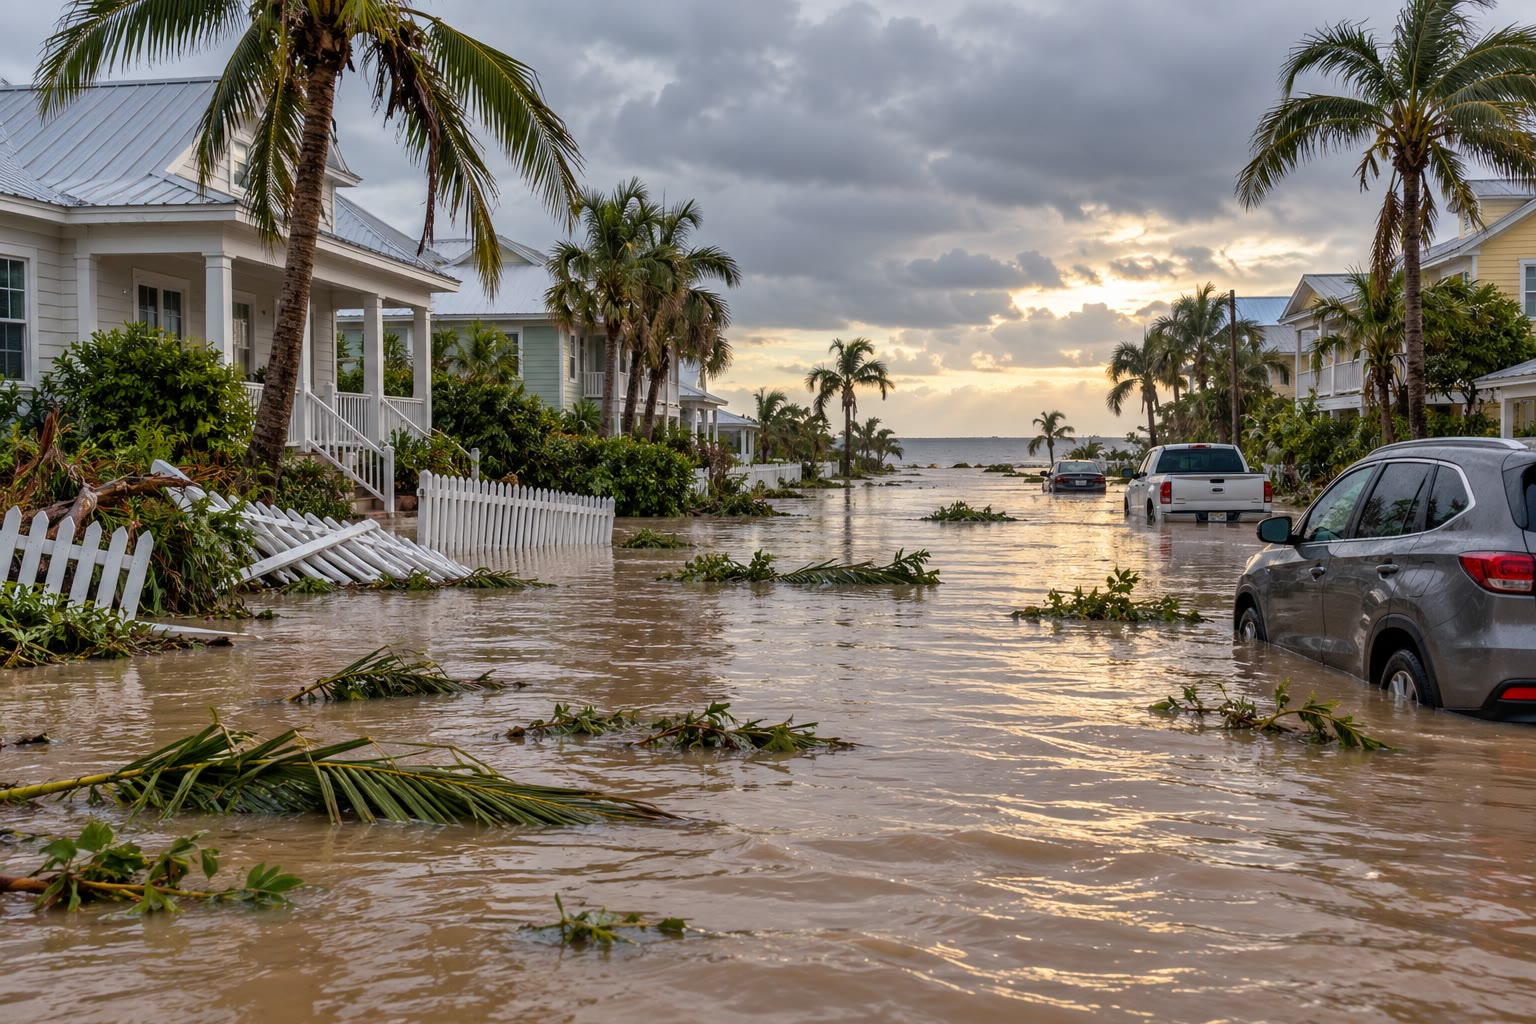
\includegraphics[width=0.7\linewidth]{images/book2/ai/g10-flooded-street.jpg}

{\small \omterm{def:g10:storms-and-cyclones:storm-surge}{तूफ़ानी महोर्मि} के बाद की सुबह तट की एक गली: समुद्री जल, टूटे
ताड़ और उखड़ी बाड़ें।}
\end{omfigure}

\section{अभ्यास}

\begin{exercise}[$\star$]\label{exo:g10:storms-and-cyclones:1}
\omterm{def:g10:storms-and-cyclones:thunderstorm}{तड़ित-झंझा} और \omterm{def:g10:storms-and-cyclones:lightning}{तड़ित} की परिभाषा दीजिए। गरज की ध्वनि किससे उत्पन्न होती है?
\end{exercise}

\begin{exercise}[$\star$]\label{exo:g10:storms-and-cyclones:2}
\omterm{def:g10:storms-and-cyclones:tropical-cyclone}{उष्णकटिबंधीय चक्रवात}, उसकी \omterm{def:g10:storms-and-cyclones:tropical-cyclone}{आँख} और उसकी \omterm{def:g10:storms-and-cyclones:tropical-cyclone}{आँख की दीवार} की परिभाषा दीजिए। उसकी पवनें
कहाँ सबसे तेज़ होती हैं?
\end{exercise}

\begin{exercise}[$\star$]\label{exo:g10:storms-and-cyclones:3}
\num{70}~नॉट की सतत पवनों वाला हरिकेन \omterm{def:g10:storms-and-cyclones:scale}{सैफ़िर--सिम्पसन पैमाने} की किस श्रेणी
में है? \num{120}~नॉट वाला? \num{140}~नॉट वाला? इनमें से कौन-से
प्रमुख हरिकेन हैं?
\end{exercise}

\begin{exercise}[$\star$]\label{exo:g10:storms-and-cyclones:4}
आप एक चमक और उसकी गरज के बीच \num{9} सेकंड गिनते हैं, फिर अगली चमक के लिए \num{15}
सेकंड। हर चमक कितनी दूर थी, और क्या तूफ़ान पास आ
रहा है?
\end{exercise}

\begin{exercise}[$\star$]\label{exo:g10:storms-and-cyclones:5}
समझाइए कि \omterm{def:g10:storms-and-cyclones:thunderstorm}{तड़ित-झंझा} में किसी खेत में अकेला खड़ा पेड़ ख़तरनाक शरण क्यों है, और
उसके बजाय आपको कहाँ जाना चाहिए।
\end{exercise}

\begin{exercise}[$\star\star$]\label{exo:g10:storms-and-cyclones:6}
एक नॉट \qty{1852}{m} प्रति घंटा है। \num{64}~नॉट और
\num{137}~नॉट को \unit{m/s} और \unit{km/h} में बदलिए।
\end{exercise}

\begin{exercise}[$\star\star$]\label{exo:g10:storms-and-cyclones:7}
पृथ्वी पर हर सेकंड 44 \omterm{def:g10:storms-and-cyclones:lightning}{तड़ित-चमकें} होती हैं। एक दिन में यह कितनी हुईं, और एक
वर्ष में?
\end{exercise}

\begin{exercise}[$\star\star$]\label{exo:g10:storms-and-cyclones:8}
एक हरिकेन का केंद्रीय दाब \qty{935}{hPa} है और परिवेश का
\qty{1010}{hPa}। उसके नीचे समुद्र का दाब-उभार कितना ऊँचा है?
\end{exercise}

\begin{exercise}[$\star\star$]\label{exo:g10:storms-and-cyclones:9}
मार्गों के मानचित्र की सहायता से बताइए कि \omterm{def:g10:storms-and-cyclones:tropical-cyclone}{उष्णकटिबंधीय चक्रवात} कहाँ बनते हैं और बनने के बाद
कहाँ जाते हैं। वे ठीक भूमध्य रेखा पर क्यों नहीं होते?
\end{exercise}

\begin{exercise}[$\star\star$]\label{exo:g10:storms-and-cyclones:10}
दाब--पवन आरेख की सरल रेखा $p \approx 1031 - 1.56\,v$ है
($p$ \unit{hPa} में, $v$ \unit{m/s} में)। श्रेणी 5 की निचली सीमा, \qty{70}{m/s}, के लिए
यह कितना केंद्रीय दाब देती है? \qty{40}{m/s} के
तूफ़ान के लिए?
\end{exercise}

\begin{exercise}[$\star\star$]\label{exo:g10:storms-and-cyclones:11}
समझाइए कि \omterm{def:g10:storms-and-cyclones:tropical-cyclone}{उष्णकटिबंधीय चक्रवात} स्थल पर पहुँचते ही जल्दी कमज़ोर क्यों हो जाता है, और
ठंडे जल के ऊपर कमज़ोर क्यों होता है।
\end{exercise}

\begin{exercise}[$\star\star\star$]\label{exo:g10:storms-and-cyclones:12}
हवा में ध्वनि की चाल $\sqrt{1.4\,R\,T/M}$ है, जहाँ $R =
\qty{8.314}{J.mol^{-1}.K^{-1}}$, $T$ केल्विन में और $M =
\qty{0.02897}{kg/mol}$। इसे \qty{0}{\degreeCelsius} पर और
\qty{30}{\degreeCelsius} पर परिकलित कीजिए। \qty{9}{s} की देरी के लिए दोनों
दूरियों में कितना अंतर है? क्या ``\qty{3}{s} प्रति किलोमीटर'' का नियम पर्याप्त अच्छा है?
\end{exercise}

\begin{exercise}[$\star\star\star$]\label{exo:g10:storms-and-cyclones:13}
एक तट पर \qty{4.0}{m} की \omterm{def:g10:storms-and-cyclones:storm-surge}{तूफ़ानी महोर्मि} मापी जाती है जब \qty{940}{hPa} के
केंद्रीय दाब (परिवेश \qty{1010}{hPa}) वाला एक हरिकेन तट पर
पहुँचता है। महोर्मि का कितना भाग दाब-उभार के कारण है, और कितना
पवन के कारण? यदि वह ऊँचे ज्वार के समय पहुँचे, जो माध्य समुद्र तल से \qty{1.5}{m} ऊपर है, तो
जल माध्य समुद्र तल से कितनी ऊँचाई तक पहुँचता है?
\end{exercise}

\begin{exercise}[$\star\star\star$]\label{exo:g10:storms-and-cyclones:14}
एक \omterm{def:g10:storms-and-cyclones:tornado}{टॉरनेडो} अपने अक्ष से \qty{100}{m} पर \qty{90}{m/s} की पवनों के साथ घूमता है;
एक हरिकेन केंद्र से \qty{30}{km} दूर की \omterm{def:g10:storms-and-cyclones:tropical-cyclone}{आँख की दीवार} में \qty{60}{m/s} की
पवनों के साथ। हर स्थिति में हवा को एक चक्कर पूरा करने में कितना समय लगता है? तुलना कीजिए।
\end{exercise}

\begin{exercise}[$\star\star\star$]\label{exo:g10:storms-and-cyclones:15}
1980--2024 के 3\,888 \omterm{def:g10:storms-and-cyclones:tropical-cyclone}{उष्णकटिबंधीय चक्रवातों} में से 24 ने भूमध्य रेखा के
\qty{5}{\degree} के भीतर उष्णकटिबंधीय तूफ़ान की तीव्रता प्राप्त की, 414 ने
\qty{10}{\degree} के भीतर, और 121 ने \qty{30}{\degree} से परे। तीनों
प्रतिशत परिकलित कीजिए। भूमध्य रेखा के \qty{5}{\degree} के भीतर की पट्टी पृथ्वी की
सतह का लगभग \qty{9}{\percent} ढकती है: यदि अक्षांश का कोई महत्त्व न होता तो
आप क्या अपेक्षा करते, और आप क्या निष्कर्ष निकालते हैं?
\end{exercise}

\section{समस्या: हरिकेन का ऊष्मा इंजन}

\begin{problem}[{सप्ताहांत समस्या --- एक दिन की वर्षा से पवन की
शक्ति तक}]
\label{pb:g10:storms-and-cyclones:1}
% ledger: aoml:energy, nist:water-latent, earth:Rmean, ipcc:budget-toa (all results computed in figdata/grade-10/cyclones.py or from the rounded data below)
एक औसत हरिकेन \qty{665}{km} त्रिज्या के वृत्त पर प्रतिदिन \qty{1.5}{cm} वर्षा
करता है। \qty{2.5}{MJ/kg} की \omterm{def:g10:earth-energy-budget:latent-heat}{गुप्त ऊष्मा}, जल का
\qty{1000}{kg/m^3} घनत्व, एक दिन में \qty{86400}{s}, और एक औसत हरिकेन की
पवनों की शक्ति \qty{1.5e12}{W} लीजिए।

\medskip
\noindent\textbf{भाग I --- एक दिन की वर्षा।}
\begin{enumerate}
  \item वृत्त का क्षेत्रफल परिकलित कीजिए।
  \item उस पर एक दिन में गिरने वाली वर्षा का आयतन परिकलित कीजिए।
  \item इसे घन किलोमीटर में व्यक्त कीजिए।
  \item इसका द्रव्यमान परिकलित कीजिए।
\end{enumerate}

\medskip
\noindent\textbf{भाग II --- मुक्त हुई ऊष्मा।}
\begin{enumerate}[resume]
  \item इस जल के संघनन से एक दिन में मुक्त हुई \omterm{def:g10:earth-energy-budget:latent-heat}{गुप्त ऊष्मा} परिकलित
        कीजिए।
  \item इसे शक्ति में बदलिए।
  \item पूरी पृथ्वी लगभग \qty{1.22e17}{W} सूर्य-प्रकाश अवशोषित करती है
        (\cref{ch:g10:earth-energy-budget})। एक हरिकेन इसका कितना
        अंश मुक्त करता है?
  \item औसत अवशोषित सूर्य-प्रकाश \qty{240}{W/m^2} है। तूफ़ान के क्षेत्रफल द्वारा
        अवशोषित सूर्य-प्रकाश परिकलित कीजिए और उसकी तुलना
        तूफ़ान की \omterm{def:g10:earth-energy-budget:latent-heat}{गुप्त ऊष्मा} से कीजिए।
  \item यह तुलना इस बारे में क्या दिखाती है कि तूफ़ान की ऊर्जा कहाँ
        एकत्र हुई थी?
\end{enumerate}

\medskip
\noindent\textbf{भाग III --- जल कहाँ से आता है।}
\begin{enumerate}[resume]
  \item इस वर्षा को पोषित करने के लिए हर दिन जल का कितना द्रव्यमान वाष्पित होना चाहिए?
  \item पृथ्वी की सतह का औसत वाष्पन \qty{82}{W/m^2} ले जाता है।
        कितने क्षेत्रफल पर औसत वाष्पन तूफ़ान की \omterm{def:g10:earth-energy-budget:latent-heat}{गुप्त ऊष्मा} की आपूर्ति कर सकता
        है? तूफ़ान के क्षेत्रफल से तुलना कीजिए।
  \item \cref{ch:g10:why-clouds-form} की संतृप्ति मात्राओं की तालिका की
        सहायता से उस जल की तुलना कीजिए जो संतृप्त हवा
        \qty{28}{\degreeCelsius} पर और \qty{20}{\degreeCelsius} पर धारण करती है।
  \item समझाइए कि \omterm{def:g10:storms-and-cyclones:tropical-cyclone}{उष्णकटिबंधीय चक्रवात} केवल गरम समुद्रों के ऊपर ही क्यों बनते हैं।
  \item समझाइए कि वे स्थल के ऊपर कमज़ोर क्यों हो जाते हैं।
\end{enumerate}

\medskip
\noindent\textbf{भाग IV --- पवन।}
\begin{enumerate}[resume]
  \item एक दिन में पवनों को दी गई गतिज ऊर्जा परिकलित कीजिए।
  \item श्रेणी 3 की निचली सीमा, \num{96}~नॉट, को
        \unit{m/s} में बदलिए (\num{1}~नॉट = \qty{1852}{m/h})।
  \item समुद्र की सतह के पास हवा का घनत्व लगभग
        \qty{1.16}{kg/m^3} है। उस चाल से चलती इस हवा के एक घन मीटर की गतिज
        ऊर्जा परिकलित कीजिए।
  \item एक दिन में मुक्त हुई \omterm{def:g10:earth-energy-budget:latent-heat}{गुप्त ऊष्मा} की तुलना एक दिन में पवनों की
        ऊर्जा से कीजिए।
  \item मुक्त हुई बाक़ी ऊष्मा का क्या होता है?
  \item संघनन से मुक्त हुई ऊष्मा का कितना अंश पवन बनता है?
\end{enumerate}
\end{problem}
